\documentclass{article}
\usepackage{import}
\subimport{../}{preamble}
\begin{document}

\section{Plasmon Coupling}

% Basic introduction to charge interaction and gap modes
Both the resonant field enhancement and the confinement of a surface plasmon can be improved by bringing a second surface plasmon into close proximity. Similar to coupled harmonic oscillators and dipoles, plasmons couple together via Coulomb forces, forming normal modes of oscillation. The charge distributions of the resulting normal modes depend sensitively on the particle separation and are strongly confined to the dielectric space between metallic surfaces where charges strongly interact. These normal modes are therefore more generally known as \emph{gap plasmons} and lead to tuneable plasmon resonances \cite{huang2010, millyard2012} and significant increases in field enhancement, enabling single molecule spectroscopy \cite{mertens2013, taylor2014}.

Coupled plasmons are a feature of many metallic nano-systems with closely spaced metal-dielectric interfaces, including \gls{mim} and \gls{imi} waveguides \cite{maier2007plasmonics, lindquist2013} and systems containing multiple \glspl{mnp} \cite{maier2002, atay2004, muskens2007, huang2010, millyard2012, taylor2011, herrmann2013} or \glspl{npom} \cite{okamoto2003, daniels2005, kinnan2007, mubeen2012, mertens2013, denijs2014}. For the purposes of this work, discussion is restricted to the ideal case of coupled \glspl{lsp} between two closely spaced MNPs, closely representing the experimental system, though the description of coupling is valid for many other cases involving SPs. Furthermore, in each example of coupled systems, the physics can be reduced to interactions between neighbouring charge distributions. Understanding the simple dimer system is therefore important to fully understand more complex geometries.

\begin{figure}[bt]
\centering
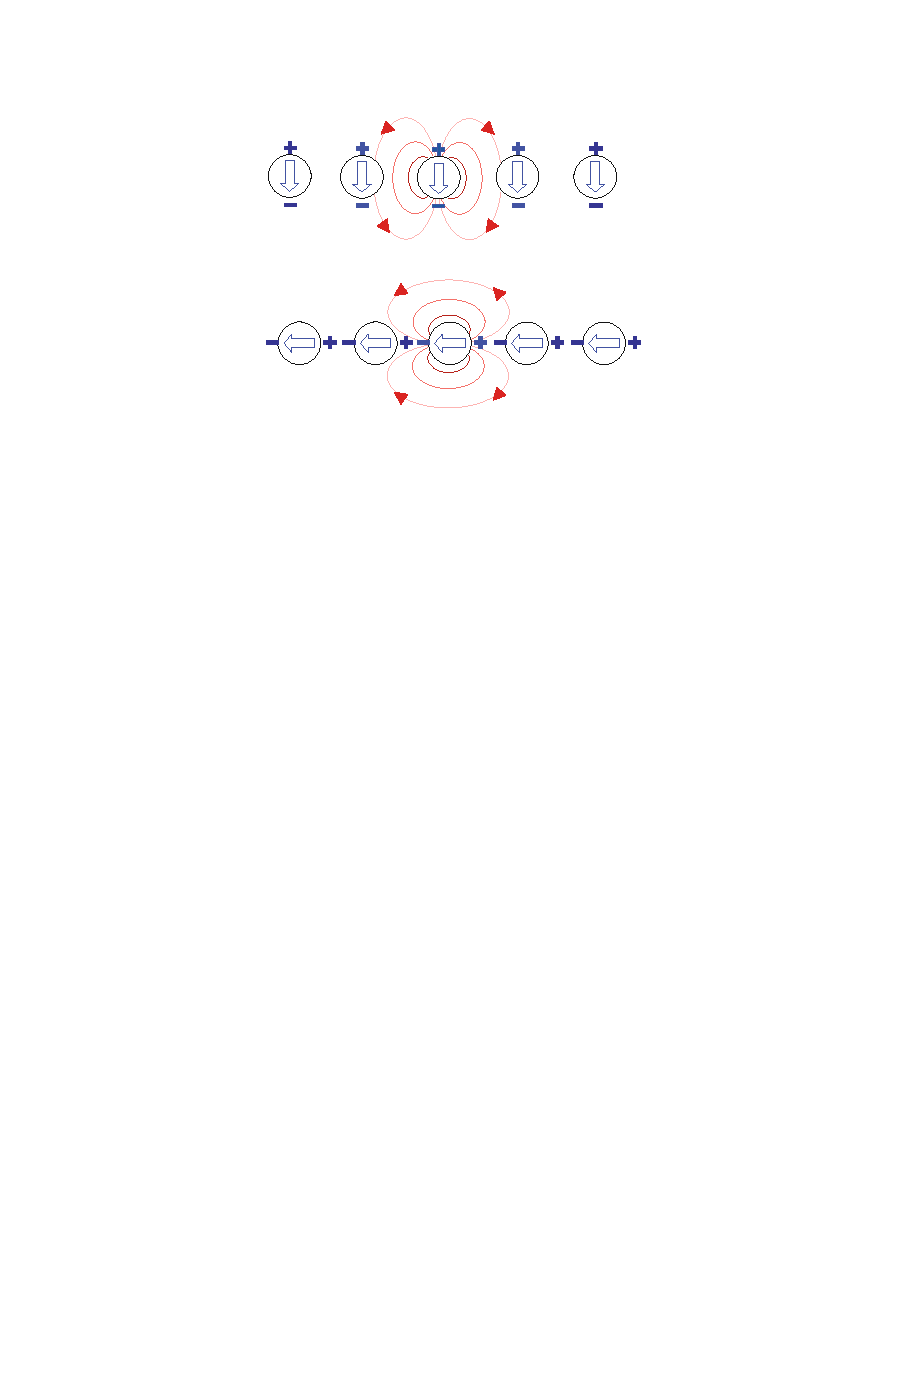
\includegraphics[width=0.45\textwidth]{figures/literature/maier_plasmonics_coupling_diagram}
\quad
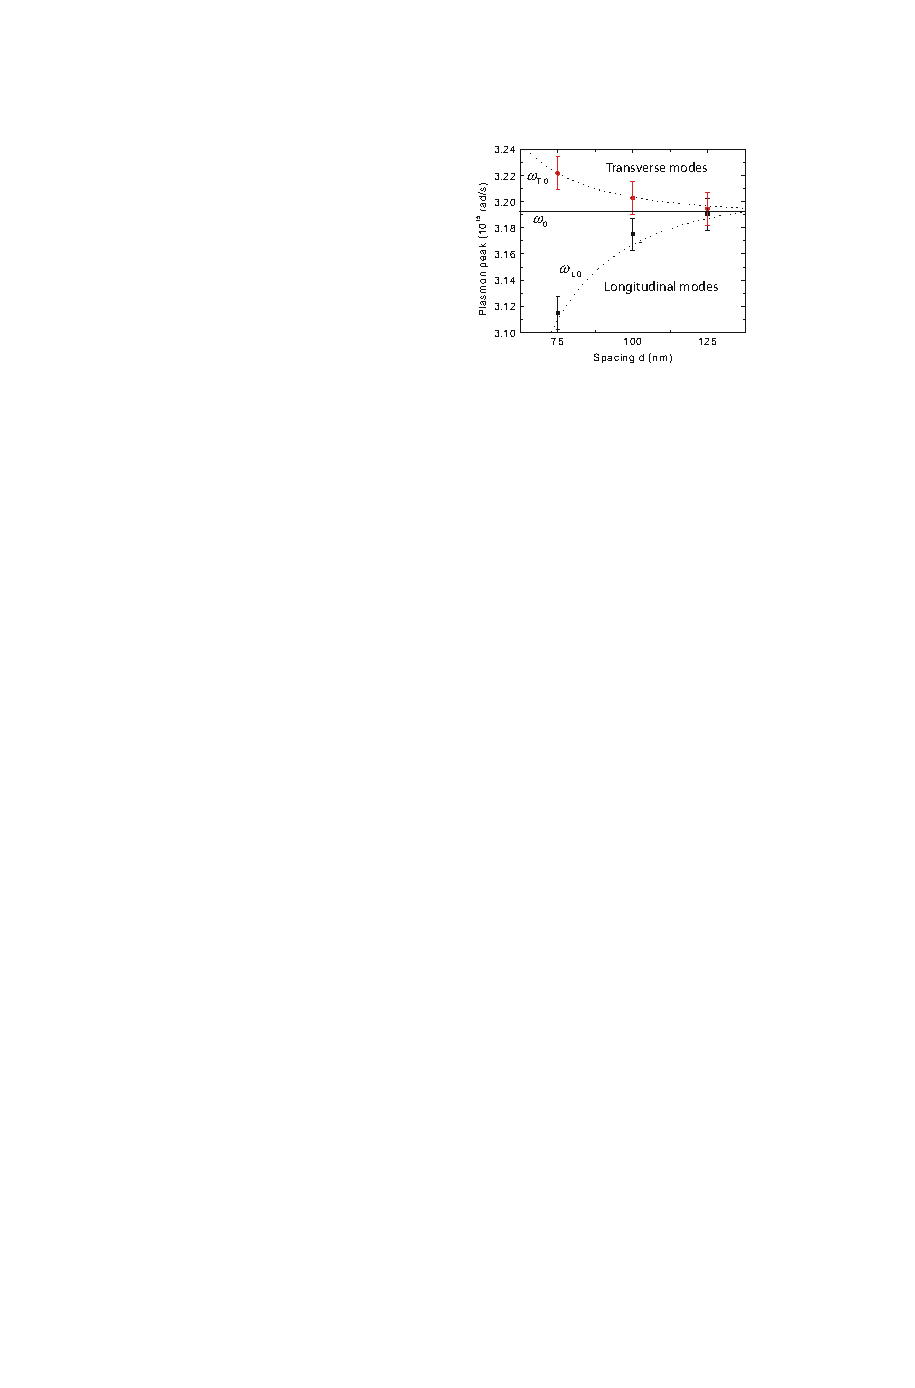
\includegraphics[width=0.45\textwidth]{figures/literature/maier_plasmonics_coupling}
\caption[Experimental and theoretical plasmon coupling]{\textbf{Experimental and theoretical plasmon coupling.} Dipolar plasmons in chains of spherical AuNPs couple depending on field orientation \cite{maier2007plasmonics} (left). Experimentally measured plasmon resonance energies in coupled AuNP chains show the gap-dependent tuning due to coupling \cite{maier2002} (right). The dotted line corresponds to a $r^{-3}$ point dipole model.}
\label{fig:maier_plasmon_coupling}
\end{figure}

In the simplest description, the Coulomb interaction between free electrons in adjacent MNPs introduces an additional coupling force, pulling charge towards the gap between metallic surfaces. A greater amount of charge accumulates on the gap-facing metallic surfaces. As particles move closer together this force grows, more strongly confining the charge and increasingly polarising the gap region. The resonance frequency of the individual plasmon mode shifts from $\omega_0$ by $\Delta\omega$ depending on the strength of coupling. The sign of $\Delta\omega$ depends on whether coupling is attractive or repulsive. Similar to coupled oscillators, the two coupling configurations (normal modes) along each axis are the in-phase and anti-phase modes. Light generally drives the free electrons of two sub-wavelength particles in phase, resulting in only an observable bonding configuration. Plasmons excited in phase along the dimer axis experience an attractive coupling force, redshifting with decreasing interparticle separation, whereas plasmons excited in phase perpendicular to the dimer axis experience repulsive coupling, blueshifting with decreasing interparticle separation. Compelling evidence for each of these modes has been seen many times, with particularly good results found using chains of AuNPs \cite{maier2002}, as shown in \autoref{fig:maier_plasmon_coupling}. In almost all cases, it is the in-phase coupled plasmons oriented along the dimer axis that are of interest.

The primary effect of plasmon coupling orientated across the dimer gap is increased confinement of the electric field to the dielectric gap medium, leading to much larger field enhancements that can be exploited for sensing. For a strongly confined gap mode there is very little field in the metal with almost all field confined to a small mode within the gap \cite{romero2006}. This is known as a plasmonic ``hot spot". Through this mechanism alone the field enhancement can be increased by more than an order of magnitude \cite{hao2004, talley2005}. Hence, in recent years, the interests of the plasmonics community have shifted from individual plasmonic nanostructures to coupled systems in order to maximise nano-optical performance. This has led to the progression into sub-nm plasmonic cavities, the study of which is a focus of this project. The development of a theoretical model for such small systems begins with the classical models of plasmon coupling with additional complexity added until quantum mechanical effects become apparent.

\subsection{Classical Models of Plasmonic Coupling}

Two analytical classical models exist to describe plasmon coupling. The first and simplest model continues the description of the dipole plasmon present in small (quasistatic) MNPs and introduces dipole-dipole interactions. The second model of plasmon hybridisation is more complex and successfully models higher order modes of charge oscillation.

\subsubsection{Dipole-Dipole Model}

\begin{figure}[bt]
\fontsize{10pt}{1em}\selectfont
\def\svgwidth{0.7\textwidth}
\subimport{./figures/}{dipole_interactions.pdf_tex}
\caption[Diagram of dipole interactions]{\textbf{Diagram of dipole interactions.} The distance between dipoles of length $D$ is $r$ with an edge-to-edge separation $d$. Configurations 1 and 3 are comparable with plasmon coupling as a result of sub-wavelength structures being driven by a single external light field. Configurations 2 and 4 are generally unphysical or non-radiative in plasmon dimers without asymmetry or phase retardation.}
\label{fig:dipole_interactions}
\end{figure}

In its simplest case, interactions between dipolar plasmons in small MNPs appear similar to dipole-dipole interactions \cite{kreibig1995optical, maier2002, gluodenis2002, rechberger2003, atay2004}, exhibiting the same behavioural dependence on separation and relative orientation with respect to the incident field. Examples of some commonly considered dipole-dipole interaction geometries are shown in \autoref{fig:dipole_interactions}. In each situation the electric field incident on a dipole $\vec{p}_1$ is perturbed by the presence of a second dipole $\vec{p}_2$ a distance $r$ away, whose fields (described by \eqref{eq:E_out}) are superimposed onto the incident field at the location of $\vec{p}_1$. The result is in an effective field given by,
\begin{subequations}
\begin{align}
	\vec{E}_{\parallel}(\vec{p}_1) &= \vec{E}_{0,\parallel} + \frac{\vec{p}_2}{2\pi\epsfs\epsdi r^3}, \label{eq:par_coupling} \\
	\vec{E}_{\bot}(\vec{p}_1) &= \vec{E}_{0,\bot} - \frac{\vec{p}_2}{4\pi\epsfs\epsdi r^3}, \label{eq:perp_coupling}
\end{align}
\end{subequations}
where $\parallel$ and $\bot$ denote the orientation of dipoles relative to the dimer axis. The sign of the second term in each equation determines the effect of coupling whilst its strength falls as $r^{-3}$ \cite{halas2011}. The polarisability of the MNP is modified by this additional interaction field, changing the frequency at which it becomes resonant.
For two dipoles aligned end-to-end ($p \parallel r$) and driven in phase, coupling is attractive (increased \vec{E}, \eqref{eq:par_coupling}), leading to a decrease (redshift) of the resonant frequency. Conversely, the interaction between two dipoles aligned side-by-side ($p \bot r$) is repulsive (decreased E, \eqref{eq:perp_coupling}), causing an increase (blueshift) of the resonant frequency. These describe the in-phase interactions between two dipole.

Anti-phase configurations, as shown in \autoref{fig:dipole_interactions}, behave in the opposite manner to the in-phase counterparts as the direction of the Coulomb force reverses. These configurations are often ignored in quasistatic dimers since light only drives in-phase oscillations. Phase retardation across the larger dimer particles can break the coupling symmetry and allow excitation of anti-phase modes, however they still have no net dipole and remain non-radiative. Electron-based techniques such as EELS are instead used to probe these `dark' modes. Using EELS with AuNP chains, the validity of the dipole approximation was confirmed, showing good agreement with the experimental data shown in \autoref{fig:maier_plasmon_coupling} \cite{maier2002}.

The dipole-dipole model is only an approximation to actual plasmonic coupling and does not adequately account for the spatial charge distribution. It can be somewhat improved by taking into account the finite particle size. Since the internal restoring force within particles, scaling as $D^3$, contributes to the potential, the interaction energy goes as $(r/D)^{-3}$ as opposed to $r^{-3}$ \cite{jain2007}. Furthermore, this quantity is redefined to better represent a dimer using the gap width, \gls{d}, as $(d/D) = (r/D)-1$. The resonant wavelength shift due to attractive coupling can then be approximated using a ``plasmon ruler" equation \cite{jain2007, ben2011},%
\footnote{The exponential approximates a more complex power law \cite{kadkhodazadeh2014scaling}.}
\begin{equation}
	\frac{\Delta\lambda}{\lambda_0} = a\exp{\left[-\frac{(d/D)}{\tau}\right]},
	\label{eq:plasmon_ruler}
\end{equation}
where $a$ is the coupling strength and $\tau$ is a decay constant. In essence, this model describes an interesting phenomenon - that plasmon coupling is scale invariant. Dimers comprised of larger particles interact more strongly for the same separation than smaller dimers. However, their relative shifts depend on how the gap size compares with the particle size. In recent years this relation still shows good agreement with experimental data but the approach remains limited to describing only dipolar modes in simple geometries \cite{muskens2007}.

\FloatBarrier
\subsubsection{Plasmon Hybridisation}

\begin{figure}[bt]
\centering
\fontsize{10pt}{1em}\selectfont
\def\svgwidth{0.98\textwidth}
\subimport{./figures/}{plasmon_dimer_hybridisation.pdf_tex}
\caption[Diagram of plasmon hybridisation between coupled plasmons in a nanoparticle dimer]{\textbf{Diagram of plasmon hybridisation between coupled plasmons in a nanoparticle dimer.} Plasmons are coupled along the dimer axis. Coupling leads to bonding and anti-bonding modes for each set of interacting $l$ modes (left). Interaction with higher order $l$ modes lowers the overall energy of lower order coupled modes (green lines). Only the bonding ($\omega_{\uparrow\uparrow}$) mode in the symmetric (homo-)dimer has a net dipole moment and is therefore observable. Cancellation of the net dipole moment means the anti-bonding ($\omega_{\uparrow\downarrow}$) mode remains optically dark. On the contrary, asymmetry in a (hetero-)dimer means both modes stay bright (right). In this case, the lower and higher energy individual modes shift to form the bonding and anti-bonding hybridised modes, respectively. This diagram is adapted from \cite{nordlander2004}.}
\label{fig:plasmon_hybridisation}
\end{figure}

A slightly more complex model, known as plasmon hybridisation, was developed to more generally explain the formation and behaviour of coupled modes \cite{prodan2003, prodan2004, nordlander2004}. In this model, plasmon resonances are mechanically modelled as resonant oscillations of an incompressible fluid confined within an equilibrium geometry \cite{prodan2004}. The plasmon resonances of a more complex particle geometry are then solved by decomposing it into coupled resonances of two simpler particle geometries \cite{prodan2003, prodan2004}. This is done in analogy with the ideas underpinning molecular orbital hybridisation and the hybridisation of quantum energy states. Using this logic, the theory equally describes the plasmon resonances of two coupled simple particle geometries \cite{nordlander2004} or a particle coupled with its image charge in a surface \cite{nordlander2004a}. Under these circumstances, the multipolar modes of each of the individual dimer particles energetically split into two hybridised modes representing the bonding (in-phase) and anti-bonding (anti-phase) configurations. This behaviour is shown in \figurename~\ref{fig:plasmon_hybridisation}.

\begin{figure}[bt]
\centering
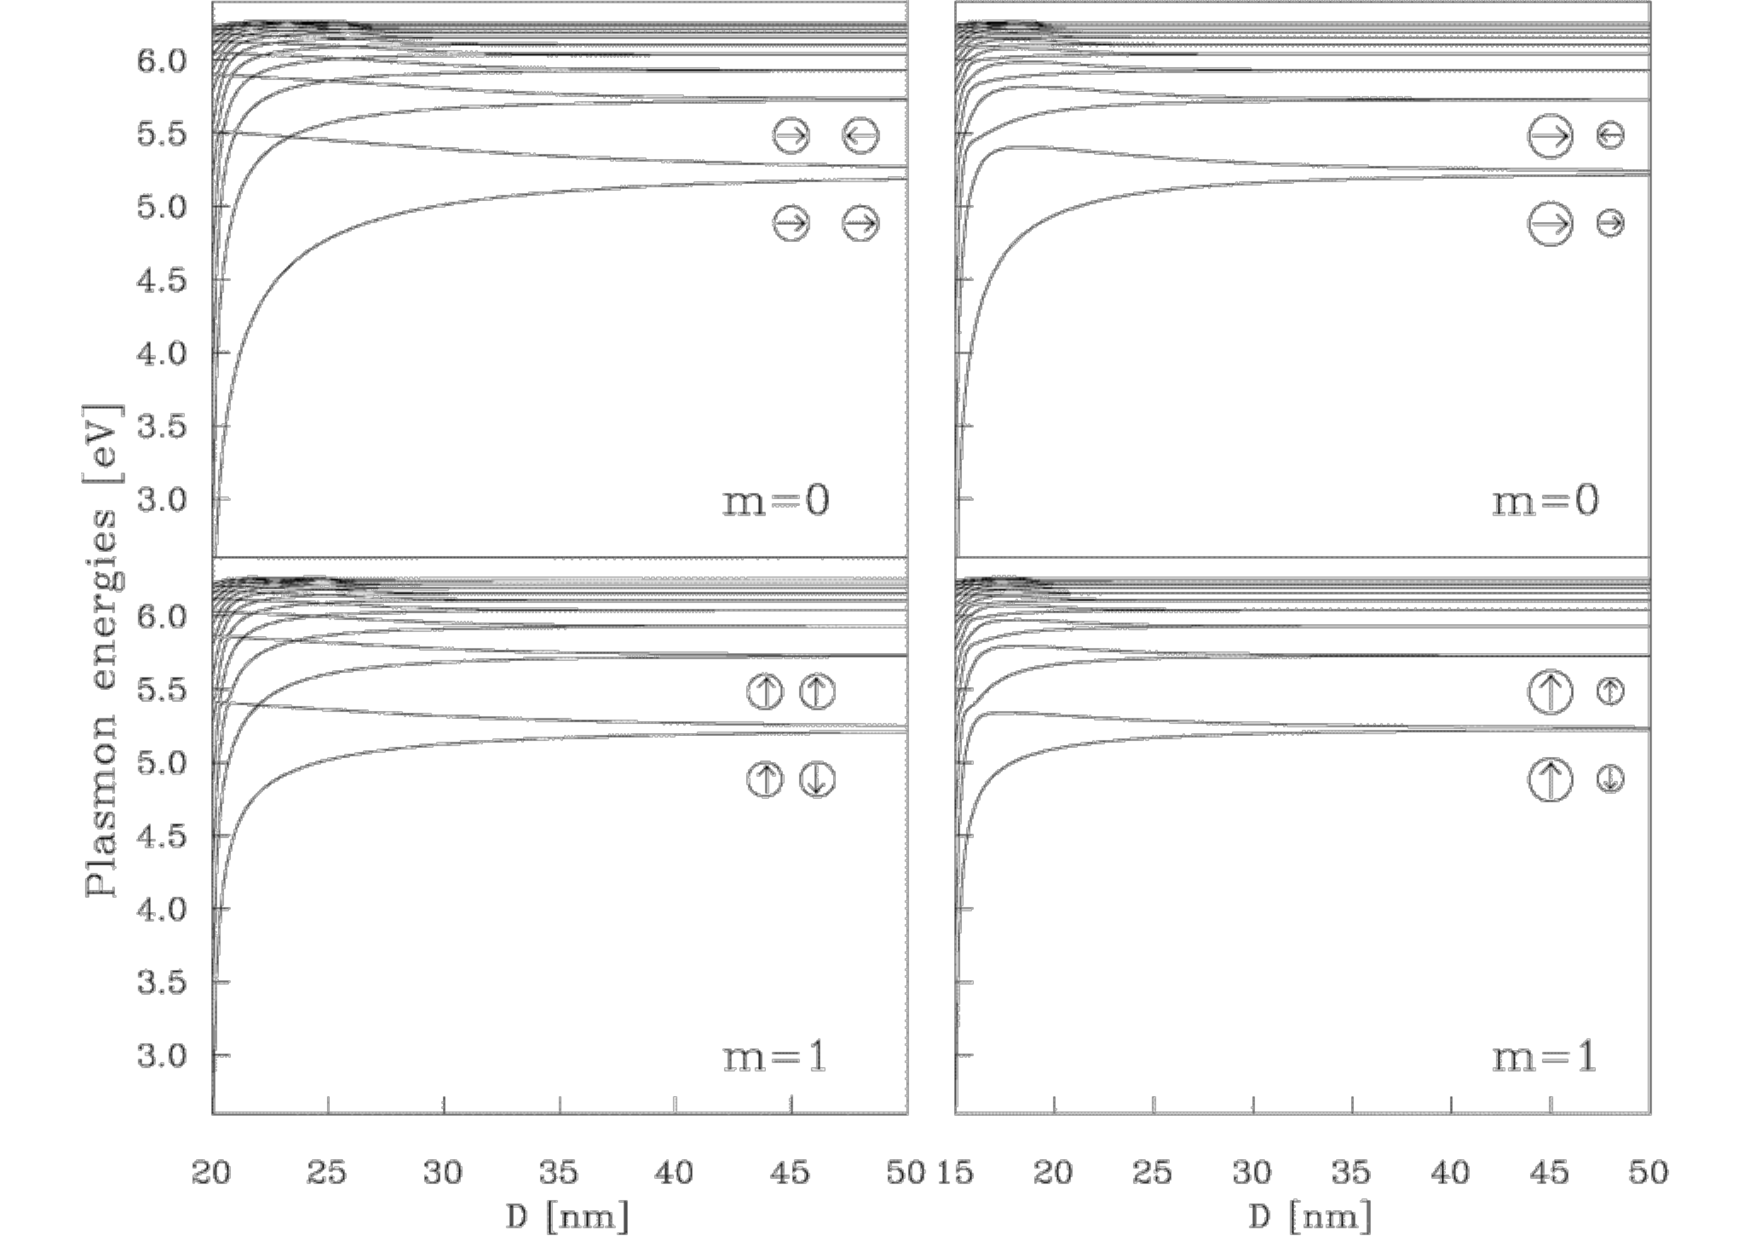
\includegraphics[width=0.7\textwidth]{figures/literature/nordlander2004}
\caption[Hybridised plasmon energy shifts for spherical AuNP dimers]{\textbf{Hybridised plasmon energy shifts for spherical AuNP dimers.} Homodimer (left) and heterodimer (right) plasmon energies are calculated in both the axial (top) and transverse (bottom) coupling configurations. Spheres are \SI{10}{nm} in diameter in the homodimer and \SI{10}{nm} and \SI{5}{nm} in the heterodimer.}
\label{fig:nordlander_ph_modes}
\end{figure}

Unlike the dipole-dipole model, plasmon hybridisation is capable of predicting higher order multipolar modes in a coupled dimer system as well as dealing with more complex geometries. It is therefore valid for describing larger dimer geometries and smaller gap sizes. As with dipole-dipole interactions, the bonding and anti-bonding hybridised modes redshift and blueshift from their initial mode positions, respectively, upon decreasing the separation. These shifts in the plasmon energies are shown in \autoref{fig:nordlander_ph_modes}. However, the addition of higher order modes to the classical description of plasmon coupling, and their interaction with adjacent modes of similar energies, modifies the rates of each mode's shift, as shown by the green lines in \autoref{fig:plasmon_hybridisation} \cite{nordlander2004}. These interactions leads to a further redshift of each affected mode, though only in the case of small gaps or larger particles once higher order modes are excited.

In each classical approach it is the resulting dipole moment of each coupled mode that dictates its radiative properties. The in-phase bonding mode exhibits a large dipole moment and strongly couples with light whereas the anti-phase anti-bonding mode has no net dipole moment in a symmetric system and thus remains dark. This remains the case until the anti-bonding dimer mode acquires a finite net dipole moment through particle asymmetry (difference material, size or shape), at which point it becomes more radiative and hence experimentally observable using optical methods. Alternatively, local excitation of specific charge distributions using EELS allows for measurement of dark modes \cite{chu2008, koh2009}. Should both bonding and anti-bonding modes be bright and gaps decrease enough that a blueshifting anti-bonding mode approaches on a higher order redshifting bonding mode, an anti-crossing will occur and modes exchange symmetry. This causes anti-bonding modes to eventually redshift into geometrical contact.

Whilst each of the previously described analytical models has found some success in describing experimentally observed plasmon coupling in simple systems, their approaches are limited in scope. Neither model directly calculates electrodynamics and solves the actual electromagnetic problem. Instead, they use analogies to similar electromechanical systems to provide a useful insight into the mechanism of plasmon coupling. The electrodynamics of a particular plasmonic problem are now often solved using computationally demanding, numerical techniques, in which the electrodynamics are solved at each boundary within a system.

\FloatBarrier
\subsection{The Dynamical Optical Response of Plasmonic Dimers: Transitioning from Capacitive to Conductive Plasmonic Coupling}
% \cite{kadkhodazadeh2013} should go in last chapter, \cite{elkhoury2014} maybe to include

Using modern numerical simulation techniques, such as the \gls{bem} and \gls{fdtd} approaches, the full separation-dependent optical response of a plasmonic dimer has been calculated as particles transition from non-interacting to coupled through into geometrical contact \cite{romero2006}. In these calculations, the lowest order plasmons hybridise, redshift and more intensely scatter as the separation decreases, with higher order modes eventually emerging. Classically, this leads to a large number of modes being present in nanometre-size gaps. The lateral confinement of the field between particles of radius $R$ separated by a gap of width $d$ is estimated as $w=\sqrt{Rd}$ \cite{romero2006}. As higher order modes become more intense, scattering from lower order modes decreases. Despite this, their field enhancement continues to rise \cite{esteban2012}. These plasmons become so confined that they no longer couple with the far-field. This behaviour continues until particles are nearly touching into geometrical contact. % check this with Jeremy's counterargument!

\begin{figure}[bt]
\centering
\fontsize{10pt}{1em}\selectfont
\def\svgwidth{0.65\textwidth}
\subimport{./figures/}{plasmon_contact.pdf_tex}
\caption[Diagram showing the emergence of charge transfer and screened bonding dimer plasmons on geometrical contact in a nanoparticle dimer]{\textbf{Diagram showing the emergence of charge transfer and screened bonding dimer plasmons on geometrical contact in a nanoparticle dimer.} The field generated by the bonding dimer plasmon (BDP) is screened from the gap by the conductive contact, forcing capacitive coupling to the outer crevices in the form of the screened bonding dimer plasmon (SBDP). The dominant charge oscillation is then the charge transfer plasmon (CTP) through the conductive bridge and across the whole structure.}
\label{fig:plasmon_contact}
\end{figure}

Once touching, bonding hybridised plasmons abruptly transition into \glspl{ctp} - charge oscillations spread across the full extent of the connected dimer. These are widely observed in geometrically contacted or overlapping plasmonic systems \cite{atay2004, lassiter2008}. A dipolar CTP emerges at lower energies (considered to be the equivalent of a monopolar dimer mode) as screened coupled plasmons are expelled out of the gap, transitioning into higher order CTPs due to their similar charge distributions \cite{romero2006, perez2010, perez2011, tserkezis2014}. Their resonances blueshift, diminishing in intensity and broadening in width as a result of significantly increased currents. The lower energies of CTPs are associated with a spatially larger dipole, as shown in \autoref{fig:plasmon_contact}, suggesting they should blueshift with increasing particle overlap. Their broad width compared with capacitively coupled plasmons is caused by dissipation in the junction and can be linked with behaviour described by \eqref{eq:dielectric_conductivity}.%
\footnote{For a spherical MNP dimer with a \gls{bdp} the corresponding CTP modes are typically labelled as the CTP and CTP$^\prime$. The CTP$^\prime$ is often labelled as the \gls{sbdp} due to similarities in charge distribution.} 

\begin{figure}[bt]
\centering
%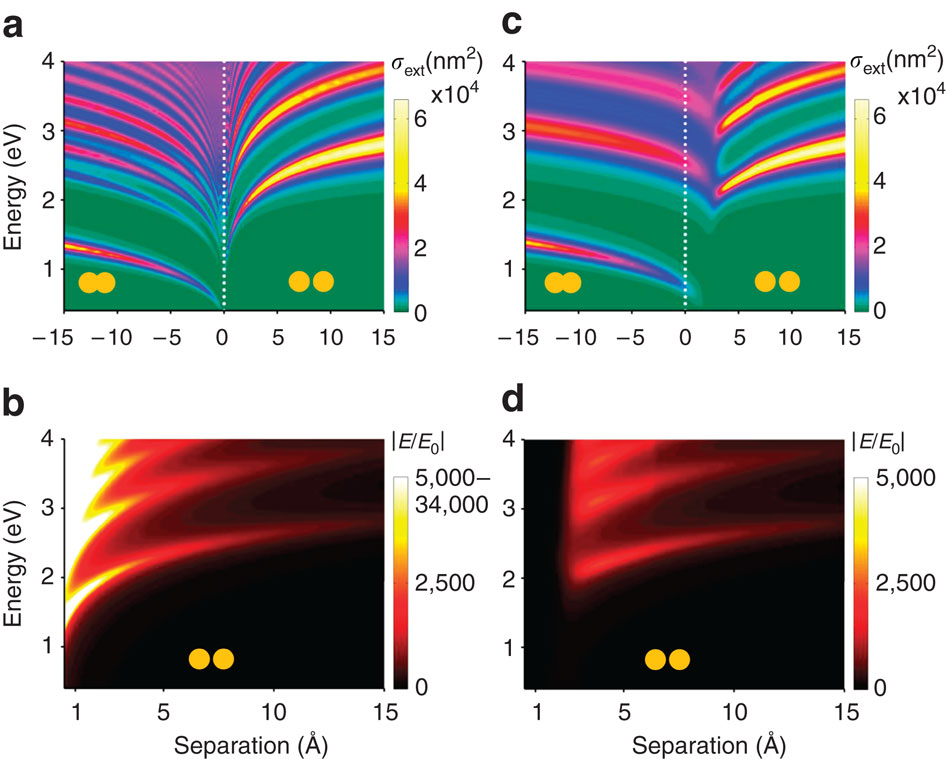
\includegraphics[width=0.7\textwidth, clip=true, trim=0 412 0 45]{figures/literature/ncomms1806-f4}\\
%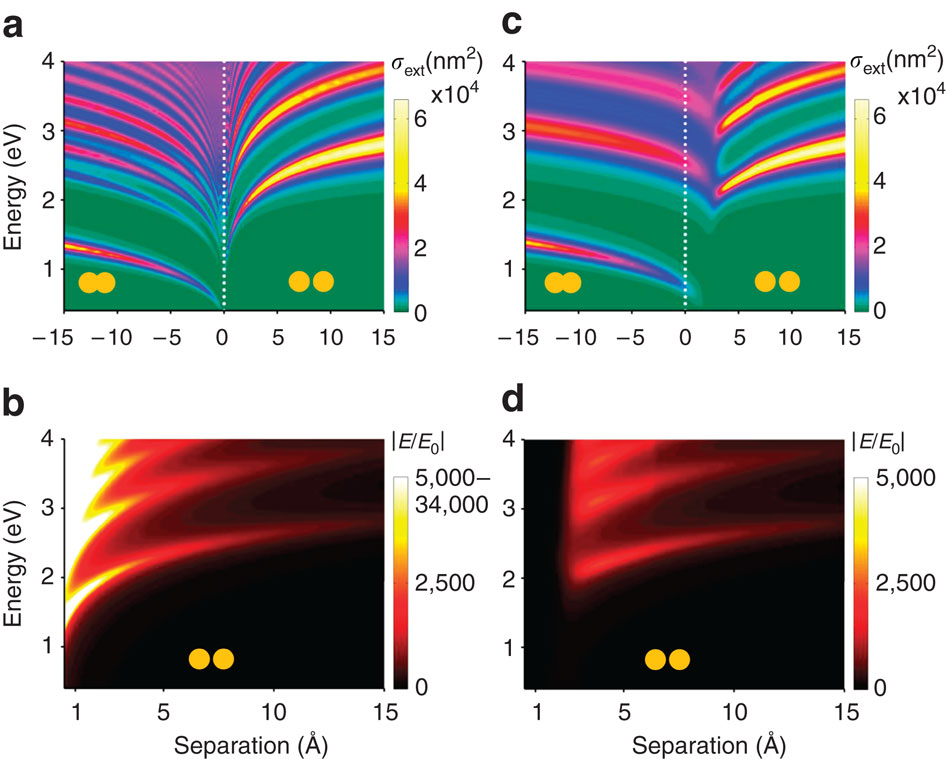
\includegraphics[width=0.7\textwidth, clip=true, trim=0 0 0 735]{figures/literature/ncomms1806-f4}
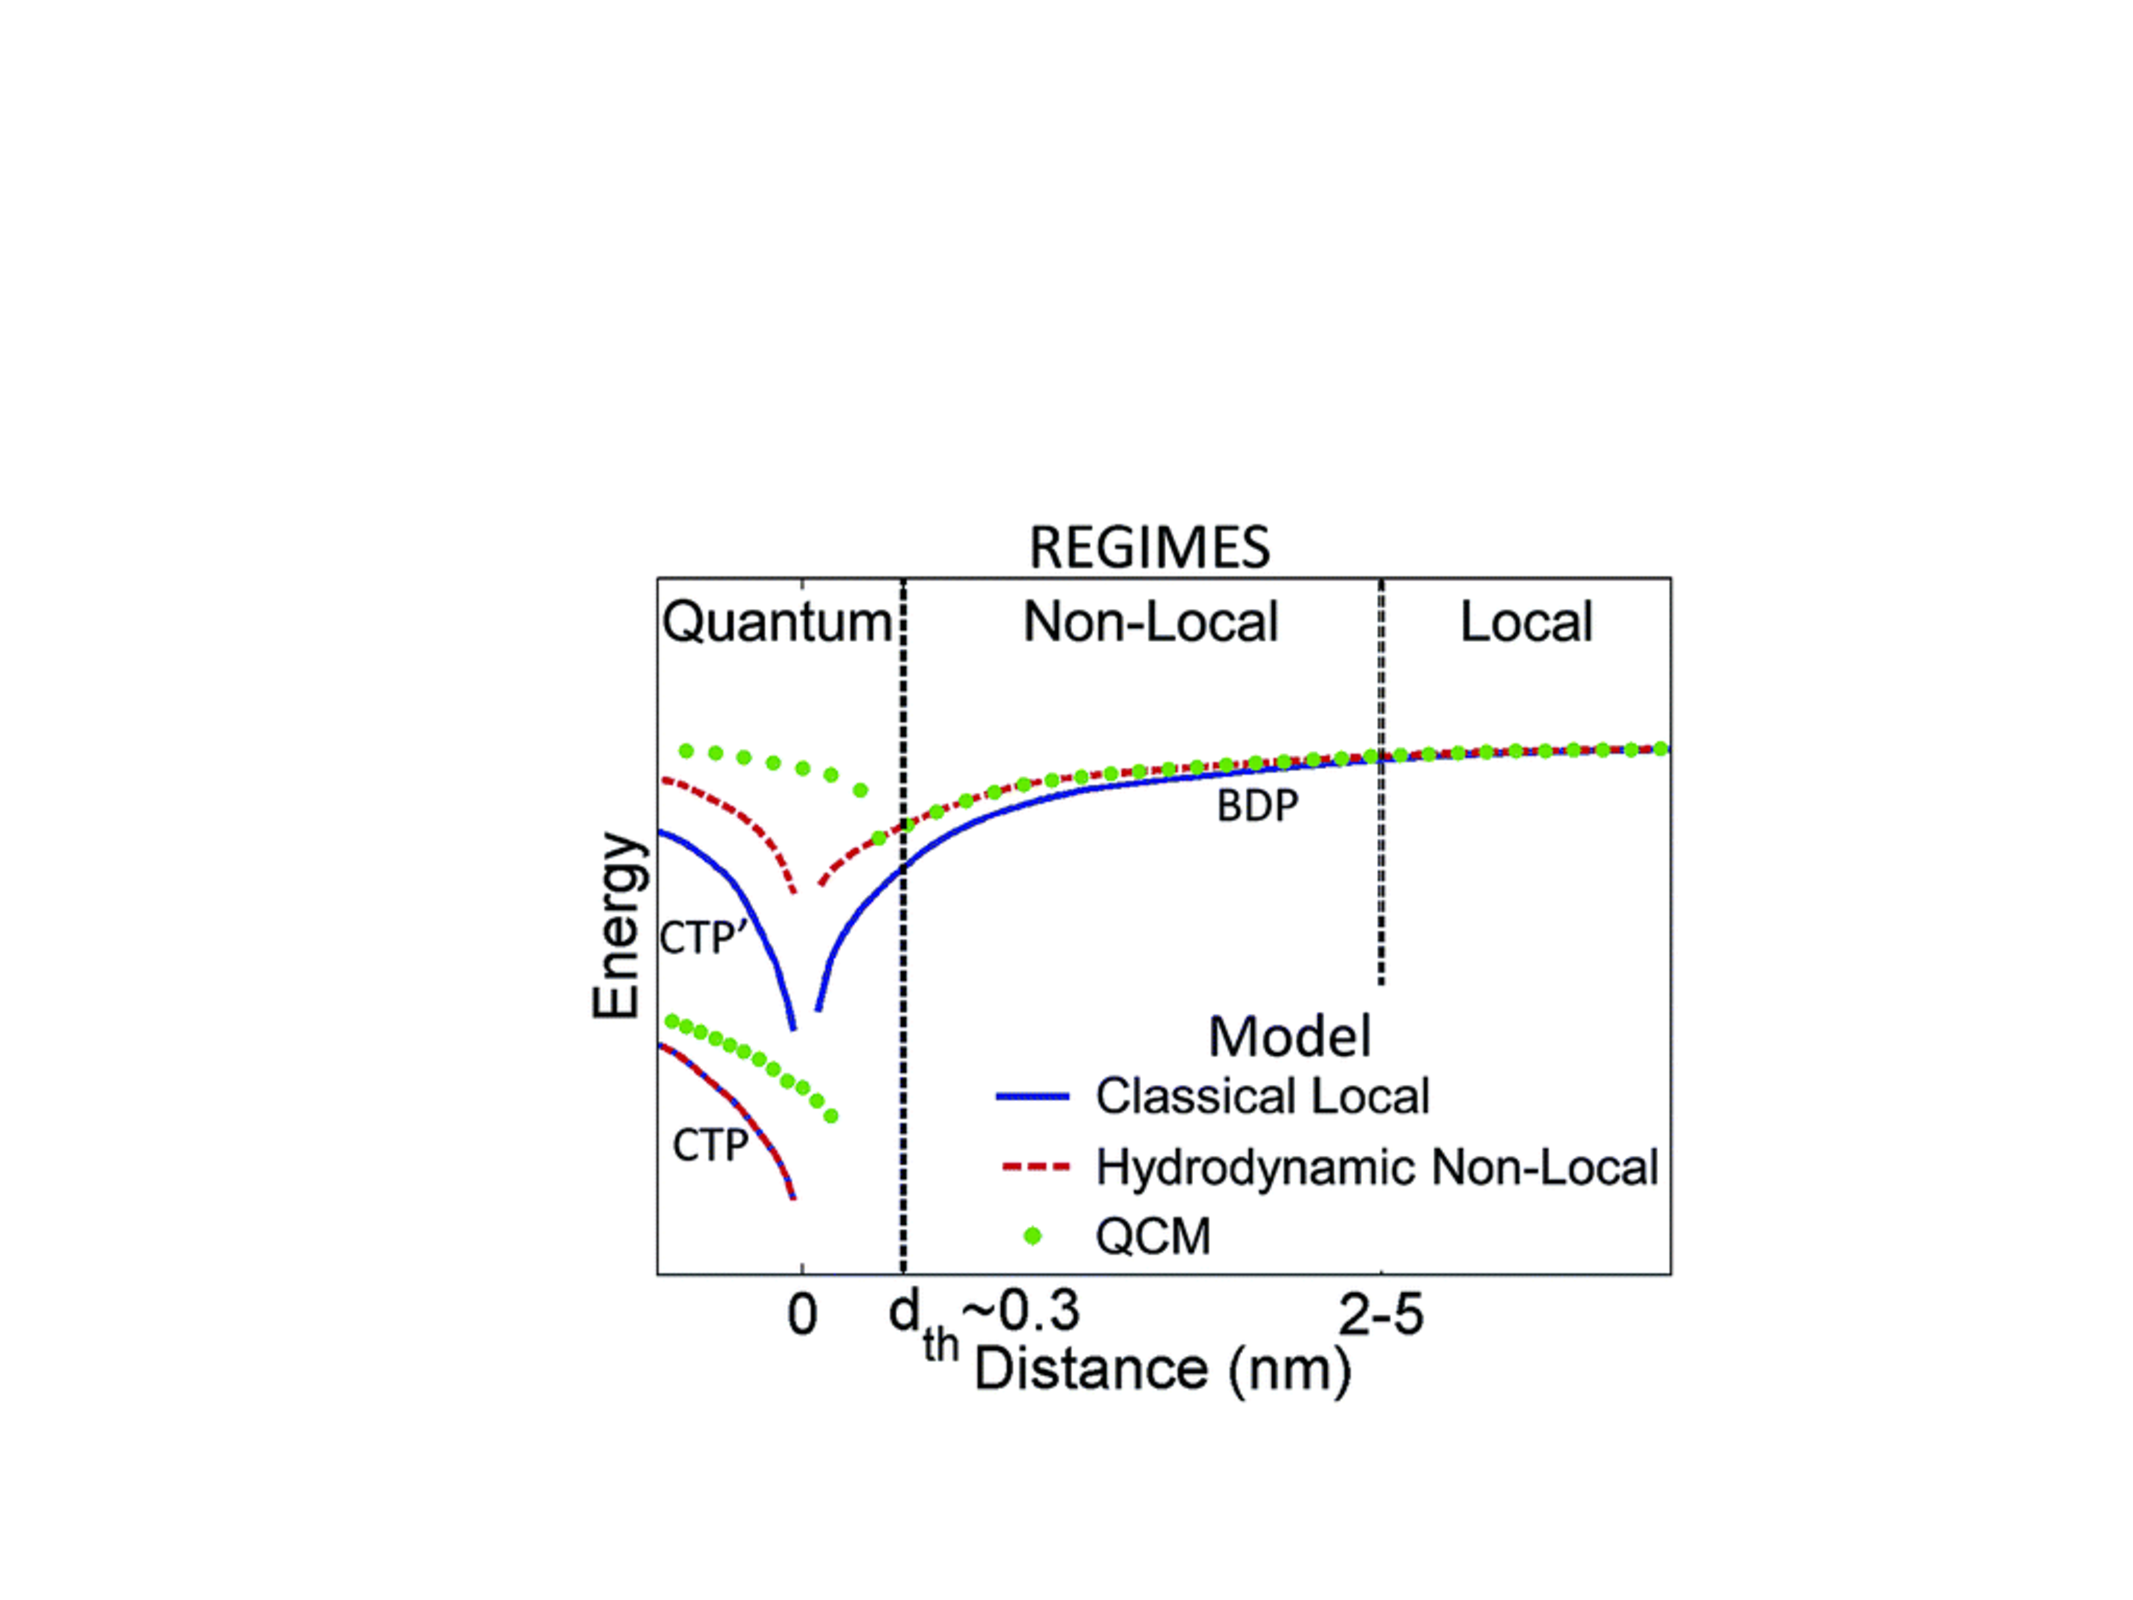
\includegraphics[width=0.5\textwidth]{figures/literature/esteban2015a}
\caption[Calculated plasmon energies of a spherical AuNP dimer as a function of gap separation using a number of computational models \cite{esteban2015}]{\textbf{Calculated plasmon energies of a spherical AuNP dimer as a function of gap separation using a number of computational models \cite{esteban2015}.} The classical local approach is valid for separations greater than \SI{2}{nm}. Below this non-locality smooths the gap and adequately describes mode behaviour until \SI{3}{\angstrom}. At this point quantum models must be used. Figure taken from \cite{esteban2015}.}
\label{fig:model_comparison}
\end{figure}

Classical predictions of plasmon coupling break down in small, sub-nm gaps where the continuum of excited higher order modes redshift to a singularity as $d\rightarrow0$, and the field enhancement increases infinitely. This behaviour is completely unphysical and is rectified once non-locality and quantum mechanical effects are considered. A comparison of the models taking these effects into account is shown in \autoref{fig:model_comparison}. Quantum mechanical effects begin to affect plasmon coupling under two conditions - either the particles become sufficiently small that non-local quantum effects (finite, non-negligible electron wavefunction spill-out from the particle) become important or the gap size decreases to scales on which quantum tunnelling and non-locality of the gap surfaces can no longer be ignored.

The non-local electron spill-out from metal surfaces smooths the gap geometry and consequently the spectral trends. The redshift into contact is heavily reduced compared with classical predictions since electrons move further into the metal on approach, suppressing coupling \cite{esteban2015}. Smoothing of sharp edges in the gap prevents a continuum of higher order modes, which become harder to excite, leaving only the most fundamental dimer modes.
Screening of the coupled modes and the emergence of CTPs prior to geometrical contact are predicted only once quantum charge transfer effects are accounted for. The onset of quantum tunnelling means charge is transported across the gap without requiring geometrical contact. This is soon after followed by a quantum conductive change transport regime prior to returning to a classical description of plasmonics. These two effects, due to their significance in sub-nm dimer gaps, are considered in more detail.

\FloatBarrier
\subsubsection{Quantum Charge Transport: Electron Tunnelling and Ballistic Transport}

\begin{figure}[bt]
\centering
\fontsize{10pt}{1em}\selectfont
\def\svgwidth{0.65\textwidth}
\subimport{./figures/}{quantum_transport.pdf_tex}
\caption[Diagram of quantum charge transport between two reservoirs of free electrons]{\textbf{Diagram of quantum charge transport between two reservoirs of free electrons.} If the Fermi energy of electrons is below the barrier potential (1) then there is a finite transmission probability $T(E_F)$ of tunnelling through the barrier. If the Fermi energy becomes larger than the potential barrier (2) then electrons are free to move through a quantised number of conducting channels of conductance $2e^2/h$.}
\label{fig:quantum_tunnelling}
\vspace{-10pt}
\end{figure}

The quantum charge transport properties of a system consisting of two reservoirs of free electrons separated by a potential barrier are determined by comparing the height of the potential barrier to the Fermi energy of each reservoir. For two metals separated by an insulating gap the potential barrier will, in general, be larger than the Fermi level. Classically, electrons with energies below the potential barrier cannot reach the other side. Electrons can only conduct through via quantum tunnelling, in which electrons incident on thin barriers have a finite probability of passing directly through the barrier as opposed to going over it. This is shown in \autoref{fig:quantum_tunnelling}.

\begin{figure}[bt]
\centering
\begin{tikzpicture}
\fontsize{10pt}{1em}\selectfont
\node [below right] at (0,0) {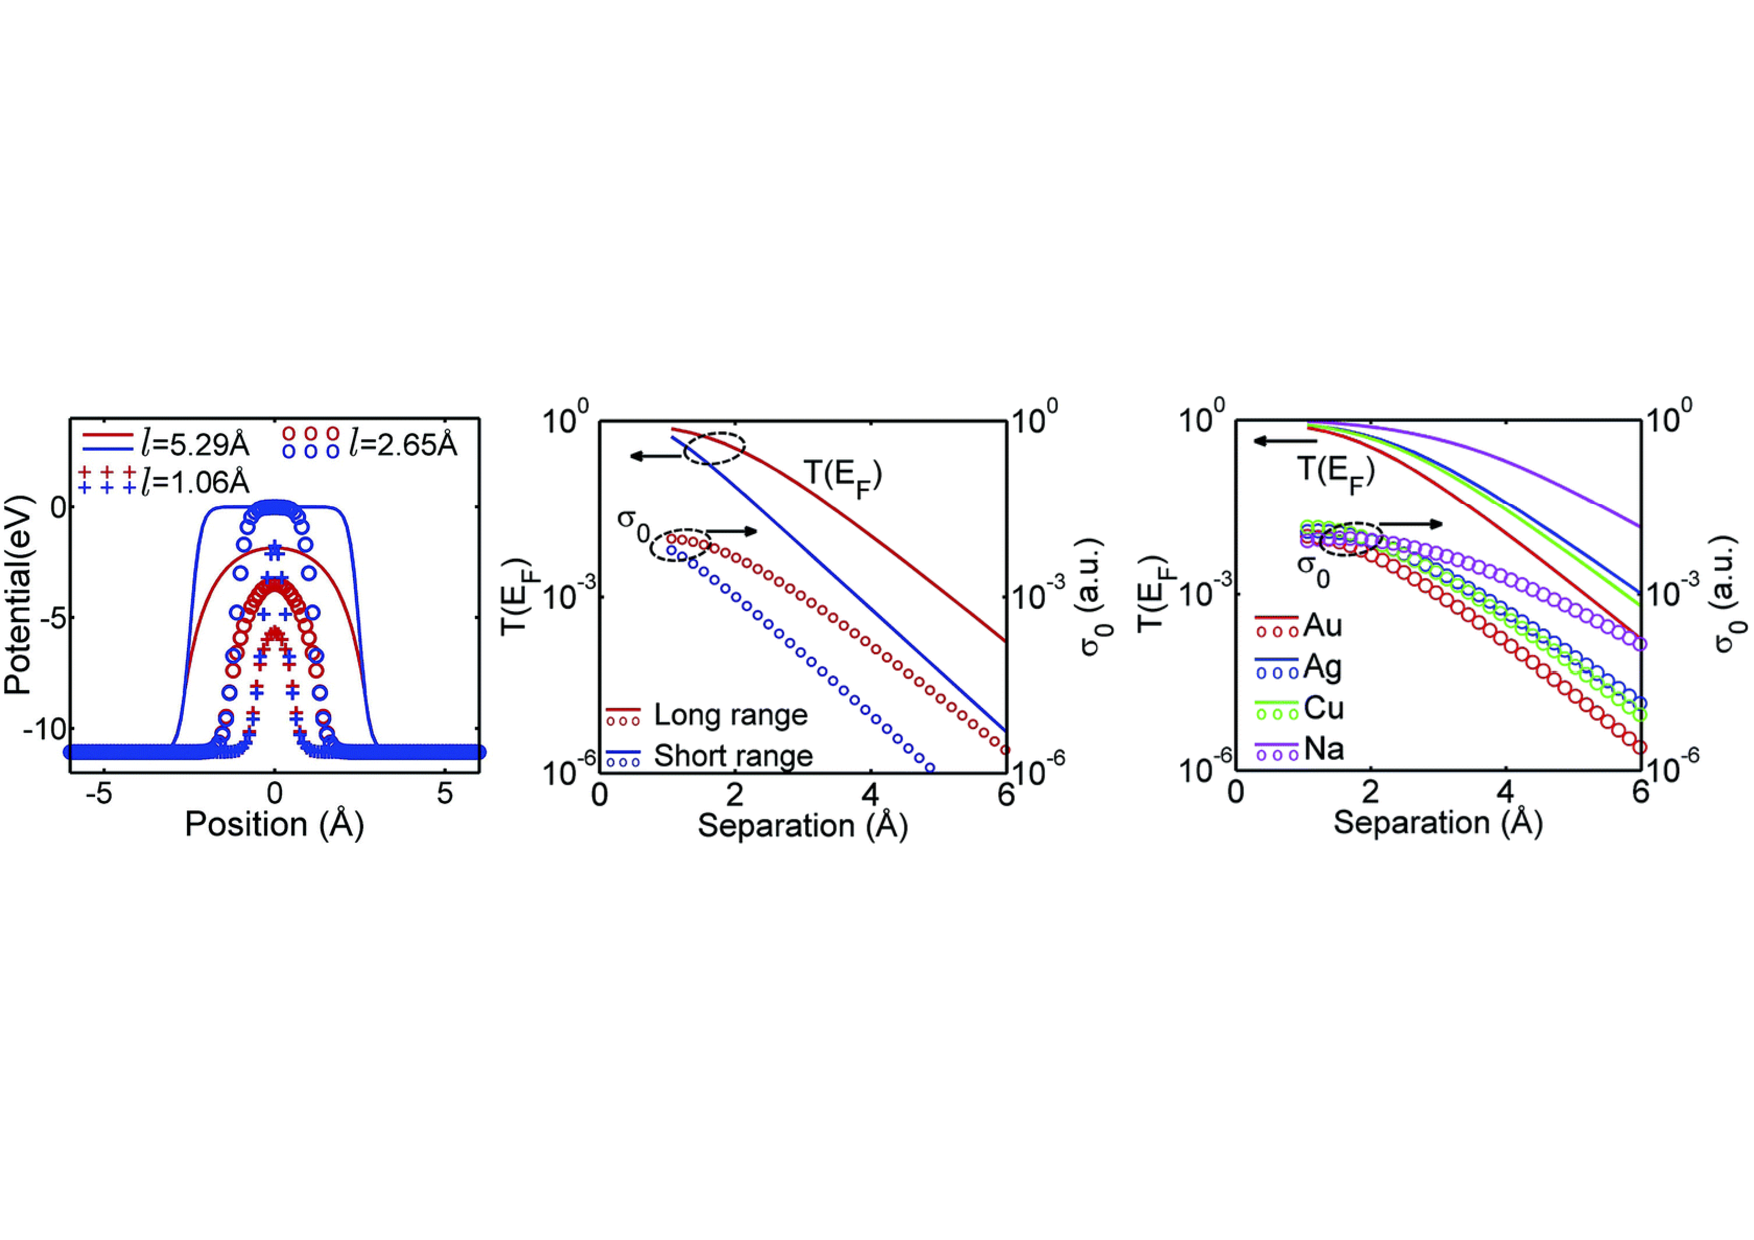
\includegraphics[width=0.95\textwidth]{figures/literature/esteban2015c}};
\node [below right] at (0,-0.05) {\textbf{a}};
\node [below right] at (4.55,-0.05) {\textbf{b}};
\node [below right] at (10.4,-0.05) {\textbf{c}};
\end{tikzpicture}
\caption[Potential barrier shapes for various gap widths and tunnelling transmission probabilities as a function of separation and material \cite{esteban2015}]{\textbf{Potential barrier shapes for various gap widths and tunnelling transmission probabilities as a function of separation and material \cite{esteban2015}.} Calculated potential barrier shapes between two Au particles as a function of separation (a) with corresponding transmissions (b). The inclusion of long-range image charge interactions is compared with a simple short-range barrier model. Realistic barrier shapes are more rounded than the simpler rectangular assumption. Overlap between rounded potential edges decreases the barrier height with reduced separation. Tunnelling increases exponentially as the gap width reduces, with increased tunnelling caused by the smaller rounded barriers. Transmission depends on the work function of a material with differing transmission probabilities at a given separation (c).}
\label{fig:esteban_tunnelling}
\end{figure}

The potential barriers and transmission probabilities of a tunnel junction between two reservoirs of Au are shown in \autoref{fig:esteban_tunnelling}. In a simplistic model, the potential layout is considered as a 1D rectangular barrier and the tunnelling probability increases exponentially with decreasing barrier width, $d$, going as $T = \e^{-\beta d}$, where $\beta$ is a decay parameter \cite{griffiths2005introduction}.%
\footnote{For a simple rectangular barrier of height $V_0$ the transmission $T=\left|t\right|^2$ is given by, $T=\e^{-2\sqrt{\frac{2m}{\hbar^2}(V_0 - E)}d}$.}
Many different mathematical descriptions of this phenomena exist \cite{simmons1963generalized, blanco2006stm}, especially after the invention of STM, that predict the conductance and resulting current density as electrons tunnel through an arbitrary potential landscape. This is in part due to the large number of parameters that influence tunnelling (e.g.\ work function, barrier potential, barrier shape, applied bias, temperature, charge hopping \cite{blanco2006stm}) and the extension of it into 3D gap morphologies, however the exponential decay is always present.%
\footnote{At least within a low bias approximation, which is generally valid in the context of this thesis.}
The current density is therefore expected to follow \cite{tan2014},
\begin{equation}
	J = J_0 \e^{-\beta d},
\end{equation}
where $J_0$ is a saturation current density. This behaviour holds for large gap sizes but begins to fail in small (\SI{2}{\angstrom}) gaps where the rectangular barrier shape assumption no longer holds (\autoref{fig:esteban_tunnelling}a,b). The barrier height begins to decrease with separation on overlap of the rounded edges. Tunnelling then becomes even more likely as the separation decreases. Since the transmission depends on the Fermi energy of free electrons in a material and the potential of the barrier region in between, different materials have different tunnelling responses. For example, tunnelling is far stronger in Na than in Au (\autoref{fig:esteban_tunnelling}c) \cite{esteban2015}. Finally, the current generated by tunnelling depends on the number of tunnelling channels available in a junction and the transmission coefficient of each channel \cite{zuloaga2009}. % how to determine the number of channels?

Once the barrier falls below the Fermi level (at $\sim$1--\SI{2}{\angstrom}), provided that the contact is short enough that motion is ballistic (no scattering), conduction electrons can move freely between the two reservoirs via a number of discretely quantised, 1D conduction channels under the application of an applied bias. This bias in the plasmonics case stems from the field induced by light. Each channel has a transmission probability $T(E_F)=1$ and a conductance given by $\G0 = 2e^2/h$, the conductance quantum \cite{landauer1957spatial}. The total conductance depends only on the number of open channels, a quantity depending typically on the width of the conductive region or the atomic scale contacts between reservoirs. This results in a conductance described by the Landauer formula%
\footnote{Full derivation of the Landauer equation and quantised conductance is found in the appendices.} \cite{landauer1957spatial},
\begin{equation}
G = \frac{2e^2}{h}\sum_n T_n(E_F) = n\G0, \label{eq:landauer}
\end{equation}
where $n$ is the number of transmission channels. Though still firmly in a quantum domain, ballistic transport is a form of conductive contact as opposed to a tunnelling phenomenon. Classical behaviour is only recovered if the length of the constriction increases to the point at which electrons begin to scatter or the width increases to allow many channels. In this event, the conductance is classified as diffusive with a conductance given by $G=\sigma A/d$.

\subsubsection{Quantum Charge Transport in Plasmonic Nanogaps}

The effects of quantum charge transport were first predicted in small ($R<\SI{2}{nm}$) NaNPs using full quantum mechanical, time-dependent (TD) \gls{dft} \cite{zuloaga2009}. Since these calculations consider the behaviour of each electron, they are currently limited in complexity to small systems containing less than 2000 electrons. Quantum effects in larger metallic nanostructures are predicted by the \gls{qcm}, a classical model which includes the effects of non-locality and uses an effective gap dielectric function that takes conductivity into account. Quantum effects are then predicted by inserting pre-calculated conductivity values from TDDFT \cite{esteban2012}. Both the QCM and TDDFT show agreement on the effects of tunnelling and conduction on plasmon coupling in NaNPs, with QCM predictions of the plasmon energies in a AuNP dimer shown in \autoref{fig:model_comparison}.

In numerical simulations, the onset of tunnelling creates a conductive bridge through which electrons can transmit during each half optical cycle. Tunnelling electrons neutralise some of the accumulated surface charge on the gap-metal interfaces, lessening the local capacitive interaction and reducing the rate of redshift. Coupled plasmons begin to be expelled from the gap and the field enhancement drastically falls \cite{zuloaga2009, esteban2012}. This is the screening effect and signifies entry into the \emph{crossover} regime \cite{zuloaga2009}. At these separations, typically \SI{5}{\angstrom} in Na, the barrier remains above the Fermi level. Screening prevents the formation of an arbitrarily large charge density around the gap and the divergence of plasmon resonances, preparing the gap for a progressive transition into conductive contact.

\begin{figure}[bt]
\vspace{-5pt}
\def\svgwidth{0.9\textwidth}
\fontsize{10pt}{1em}\selectfont
\subimport{./figures/}{charge_transfer_quantum_model.pdf_tex}
\caption[Diagram of the charge transfer process in a nanoparticle dimer]{\textbf{Diagram of the charge transfer process in a nanoparticle dimer.} The electron density is represented by the filling of the particle potential wells. Electrons are considered non-local and spill out from the gap surfaces. Long-range image charge interactions also further round the potential barrier. Tunnelling at large distances neutralises optically-driven charge accumulation on gap surfaces, reducing coupling. At smaller separations the particle Fermi level can become greater than the gap potential barrier, permitting conduction instead of tunnelling. This is the origin of gap current and CTP excitation.}
\label{fig:quantum_charge_transfer_model}
\vspace{-15pt}
\end{figure}

The conductance provided by quantum tunnelling is too small to excite CTPs, hence only screening is initially observed. Once the gap size reduces to the point at which the potential barrier falls below the Fermi level a dimer transitions into a conductive state where $T(E_F)=1$ and conductances are given by \eqref{eq:landauer}. This is the \emph{conductive} or \emph{CTP} regime, in which the free flow of electrons permits a large current through junction and enables CTP excitation \cite{zuloaga2009}. A diagram showing this changeover in conduction mechanisms is shown in \autoref{fig:quantum_charge_transfer_model}, similar to DFT calculations presented in \cite{zuloaga2009}. The increased current progressively screens and ultimately decouples gap plasmons, which blueshift into higher order CTPs. The fundamental CTP appears near to geometrical contact once the conductance rises sufficiently \cite{esteban2012, scholl2013}. Similar effects are seen in classically calculated AuNP dimers connected by a conductive bridge to mimic molecular linkers \cite{perez2010, perez2011}.

A critical gap width for such quantum conductive effects is found between 1--\SI{2}{\angstrom} for NaNPs with a similar transition occurring in AuNP dimers for gaps between \SI{1.06}{\angstrom} and \SI{2.65}{\angstrom} \cite{esteban2015}, as shown in \autoref{fig:esteban_tunnelling}a. Though quantum simulations considered only small NaNPs it is proposed that larger nanoparticle dimers could enter the quantum regime at greater separations as larger nanoparticles have more closely spaced energy levels (reduced quantum size effects) and therefore more available conductance channels \cite{zuloaga2009}. The QCM seemingly reproduces this effect with conductive effects occurring in $R=\SI{25}{nm}$ AuNP dimers at similar 2--\SI{3}{\angstrom} separations, despite the lower rate of tunnelling between Au surfaces. %This indicates that a larger conducting surface can generate a similar conductance to a smaller, more conductive junction, which is enough to exceed the critical amount of charge transfer required in one optical cycle.

\begin{figure}[bt]
\centering
\begin{tikzpicture}
\node [below right] at (0,0) {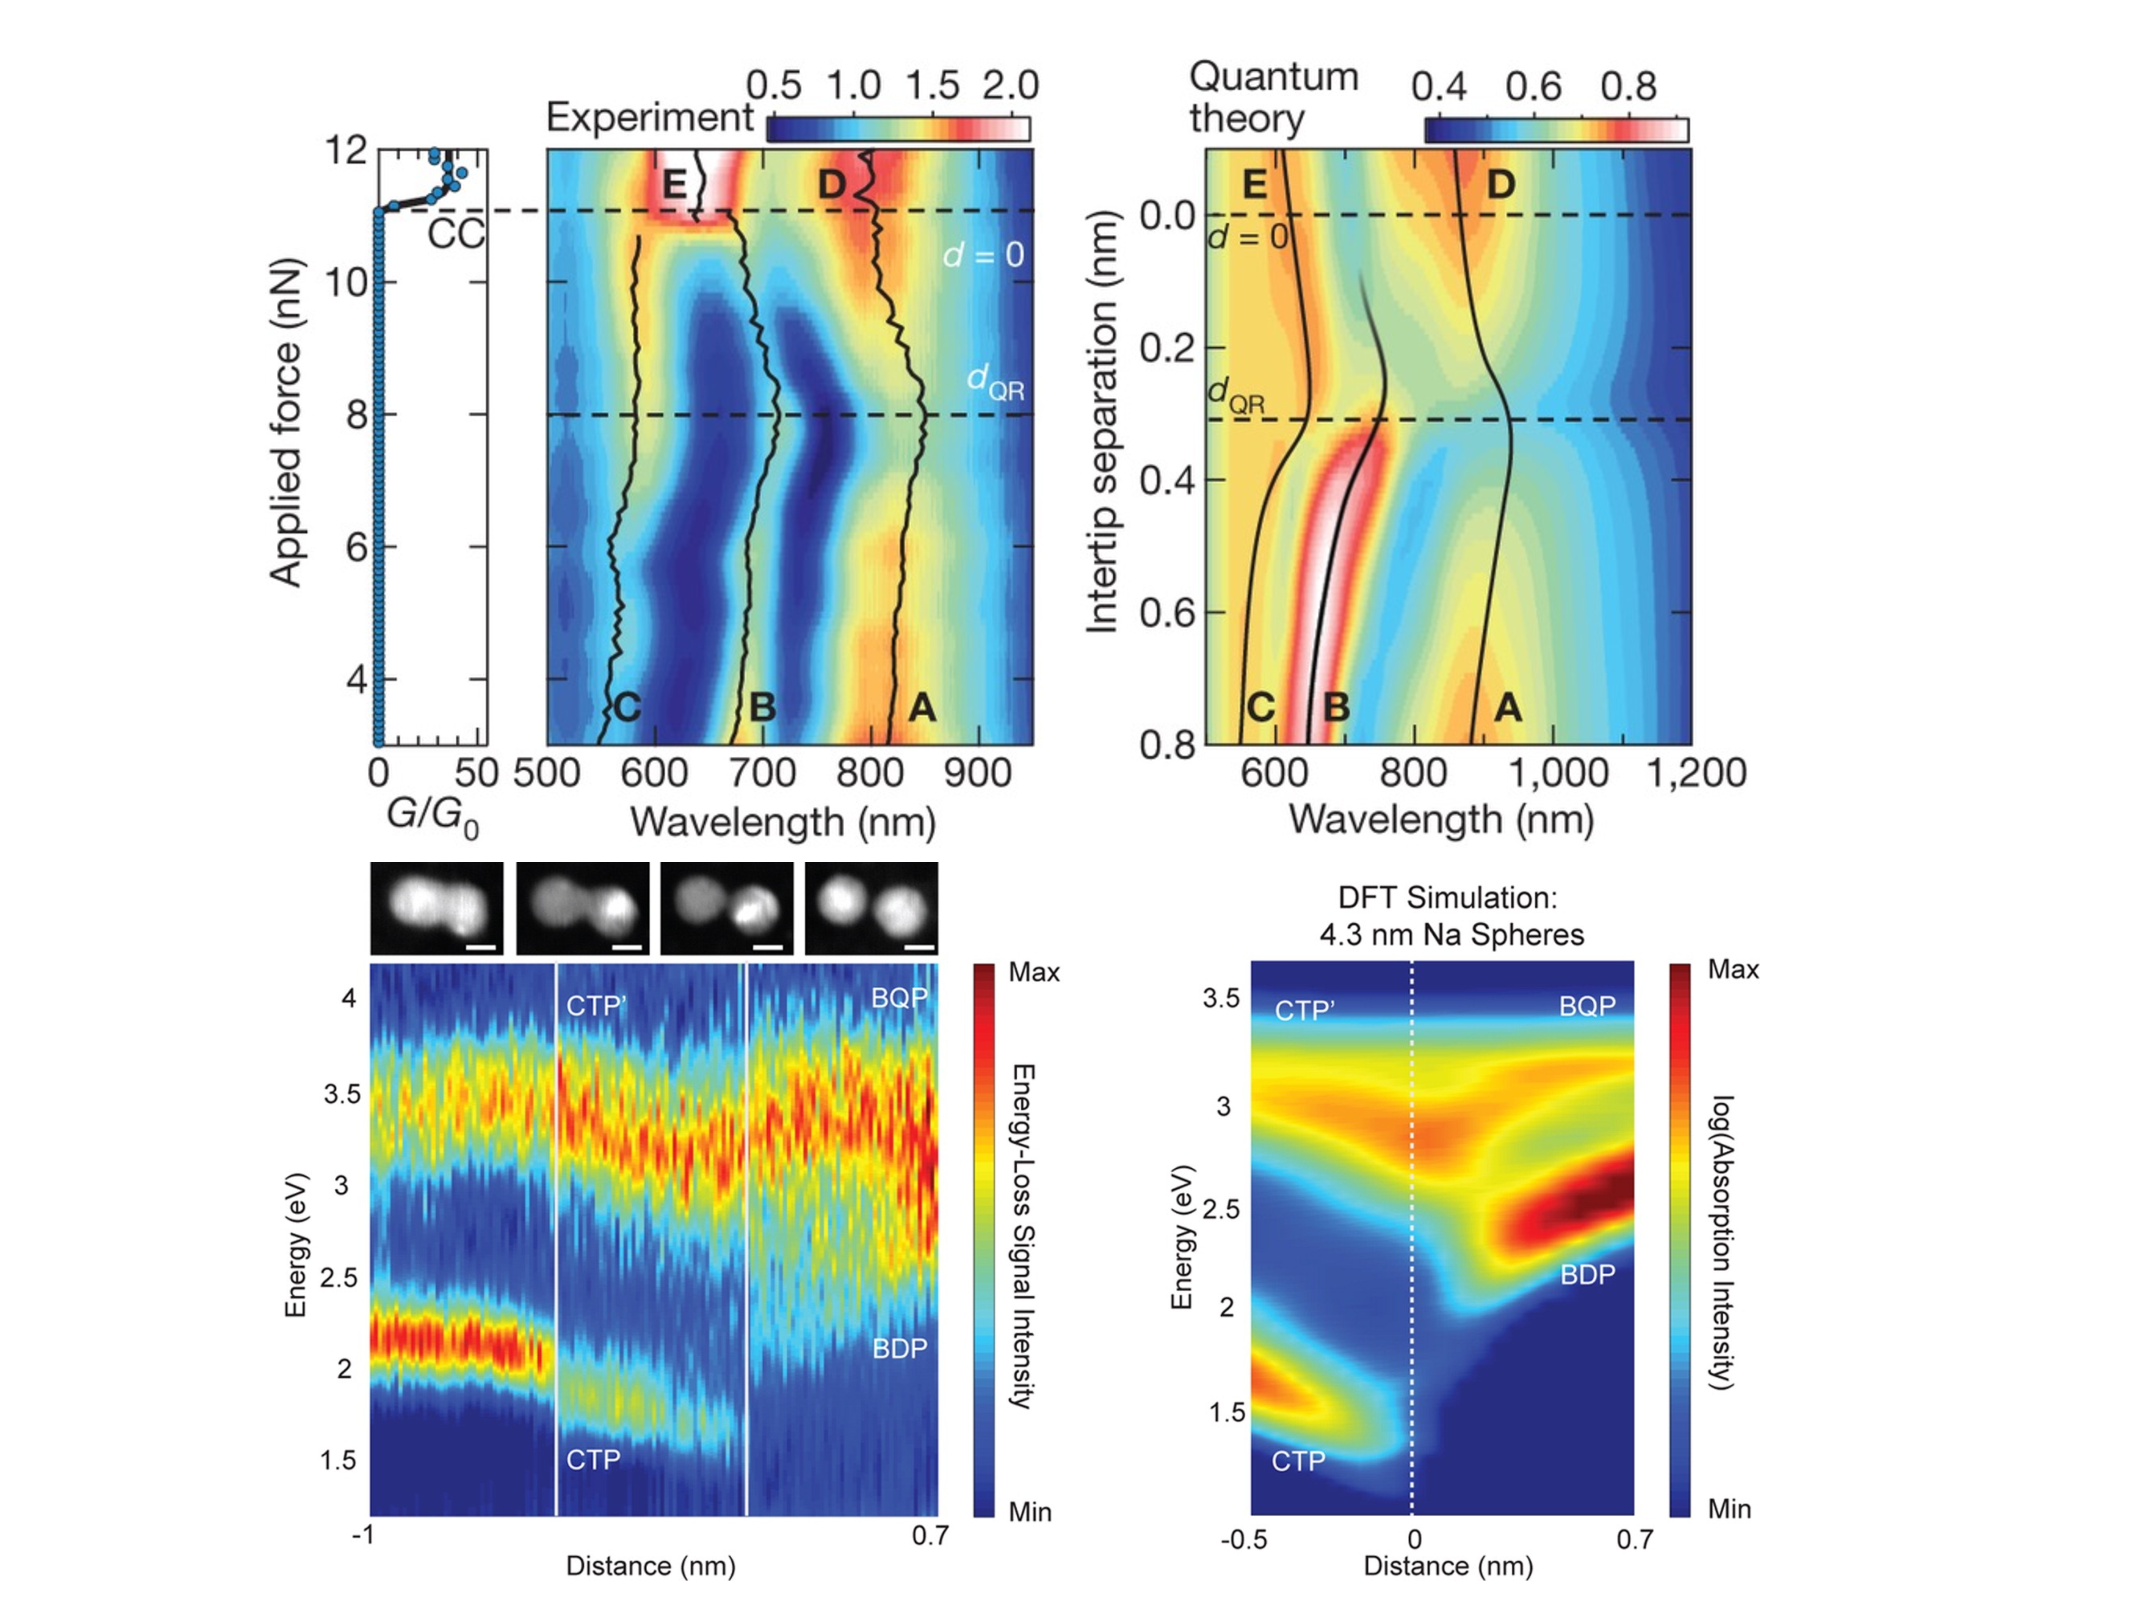
\includegraphics[width=0.7\textwidth, clip=true, trim=3 0 0 0]{figures/literature/quantum_plasmonics}};
\node [below right] at (0,-0.3) {\textbf{a}};
\node [below right] at (0,-6.6) {\textbf{b}};
{\fontsize{6.5pt}{1em}\selectfont
\node [below right] at (3.4,-11.63) {$\mathsf{<0.27}$};
\node [below right] at (2,-11.63) {$\mathsf{-0.3}$};
}
\end{tikzpicture}
\caption[Examples of experimental measurements showing the quantum regime of plasmonic coupling through direct monitoring of the plasmon resonances]{\textbf{Examples of experimental measurements showing the quantum regime of plasmonic coupling through direct monitoring of the plasmon resonances.} (a) Supercontinuum dark-field scattering measurements of two \SI{300}{nm} diameter spherical Au tips in a dimer configuration with reducing separation, transitioning below \SI{1}{nm} and into the quantum regime \cite{savage2012}. (b) EELS measurements of \SI{10}{nm} AgNPs being induced closer together by the electron beam \cite{scholl2013}.}
\label{fig:tunnelling_plasmonics}
\end{figure}

A simple estimation of this critical distance is given in \cite{savage2012}, when simulating a tip dimer with spherical Au apices. The conductive regime is said to dominate once the charge stored in a plasmon becomes less than the charge involved in charge transfer, i.e.\ the fraction of conductive charge is greater than 50\%. The tunnelling conductivity in a rectangular barrier model is,
\begin{equation}
	\sigma(d) = \frac{3k_ee^2}{4\pi h} e^{-2k_e d},
\end{equation}
where $k_e=\sqrt{2m\varphi}/\hbar$ is the electron wavenumber at the work function, $\varphi$. The distance at which this leads to a majority of charge transfer is calculated as,
\begin{equation}
	d_{QR} = \frac{1}{2k_e}\ln\left[ \frac{3k_e\lambda\alpha}{2\pi} \right],
\end{equation}
where $\lambda$ is the wavelength of the plasmon and $\alpha=1/137$, the fine structure constant. Evaluating this for Au ($\varphi=\SI{4.8}{eV}$) at an \SI{850}{nm} plasmon wavelength yields a critical separation of \SI{1.6}{\angstrom} with a conductivity of \SI{3.3e3}{S.m^{-1}}. If instead the larger conductivity from DFT is used, the equation predicts a critical gap size of \SI{3.6}{\angstrom}, similar to the \SI{3.1}{\angstrom} found in QCM spectra.

% Direct measurements
Experimental evidence of quantum transport effects in plasmonic gaps has recently been found using optical spectroscopy \cite{savage2012, cha2014, zhu2014}, EELS \cite{scholl2013}, SERS \cite{zhu2014}, photoluminescence \cite{kravtsov2014} and third-harmonic generation measurements \cite{hajisalem2014}.
Optical scattering measurements from a dynamic spherically-tipped Au AFM probe dimer clearly show the spectral signatures of quantum effects and generally agree with QCM simulations. Two coupled plasmon resonances begin to weaken during the final \SI{7}{\angstrom} of the approach into contact (\figurename~\ref{fig:tunnelling_plasmonics}a) \cite{savage2012}. Distances are determined by comparing with QCM spectra. Coupled modes blueshift upon decreasing past a \SI{3}{\angstrom} critical separation and begin to regain intensity whilst a new mode strengthens going into contact. Further experimental agreement is found in EELS measurements on \SI{10}{nm} AgNP dimers, brought together under the influence of the electron beam (\figurename~\ref{fig:tunnelling_plasmonics}b) \cite{scholl2013}. In this system the dimer exhibits simultaneous CTP excitation and coupled mode screening once $d<\SI{3}{\angstrom}$. The agreement between both experiments, the QCM and DFT calculations reinforces the idea that quantum tunnelling screens plasmon coupling and the rising conductance after ballistic conductive contact leads to the rise of CTPs. %The observation of a critical distance of \SI{3}{\angstrom} in many noble metal systems of different shapes and sizes is also intriguing and poses further questions of what exactly the conductance is at that point.

A small number of other recent experiments have also now began to report effects attributed to conduction and quantum tunnelling. Alkanedithiol molecules of various lengths have been used to discretely tune the gap separation of AuNP dimers, with attenuation and blueshifting of the BDP with molecules smaller than pentanedithiol \cite{cha2014}. Similar results are found when using intercalating \glspl{sam} \cite{tan2014}.
% Inferred measurements
Further investigations into sub-nm plasmonic gaps have also shown behaviours attributed to quantum tunnelling, though inferred from properties depending on the field enhancement as opposed to direct measurement of SPRs. A decrease in signal intensity in both the SERS peaks \cite{zhu2014} and photoluminescence \cite{kravtsov2014} in nano-gap systems, for example, are signatures of quantum tunnelling screening the coupled plasmon field.

\begin{figure}[bt]
\centering
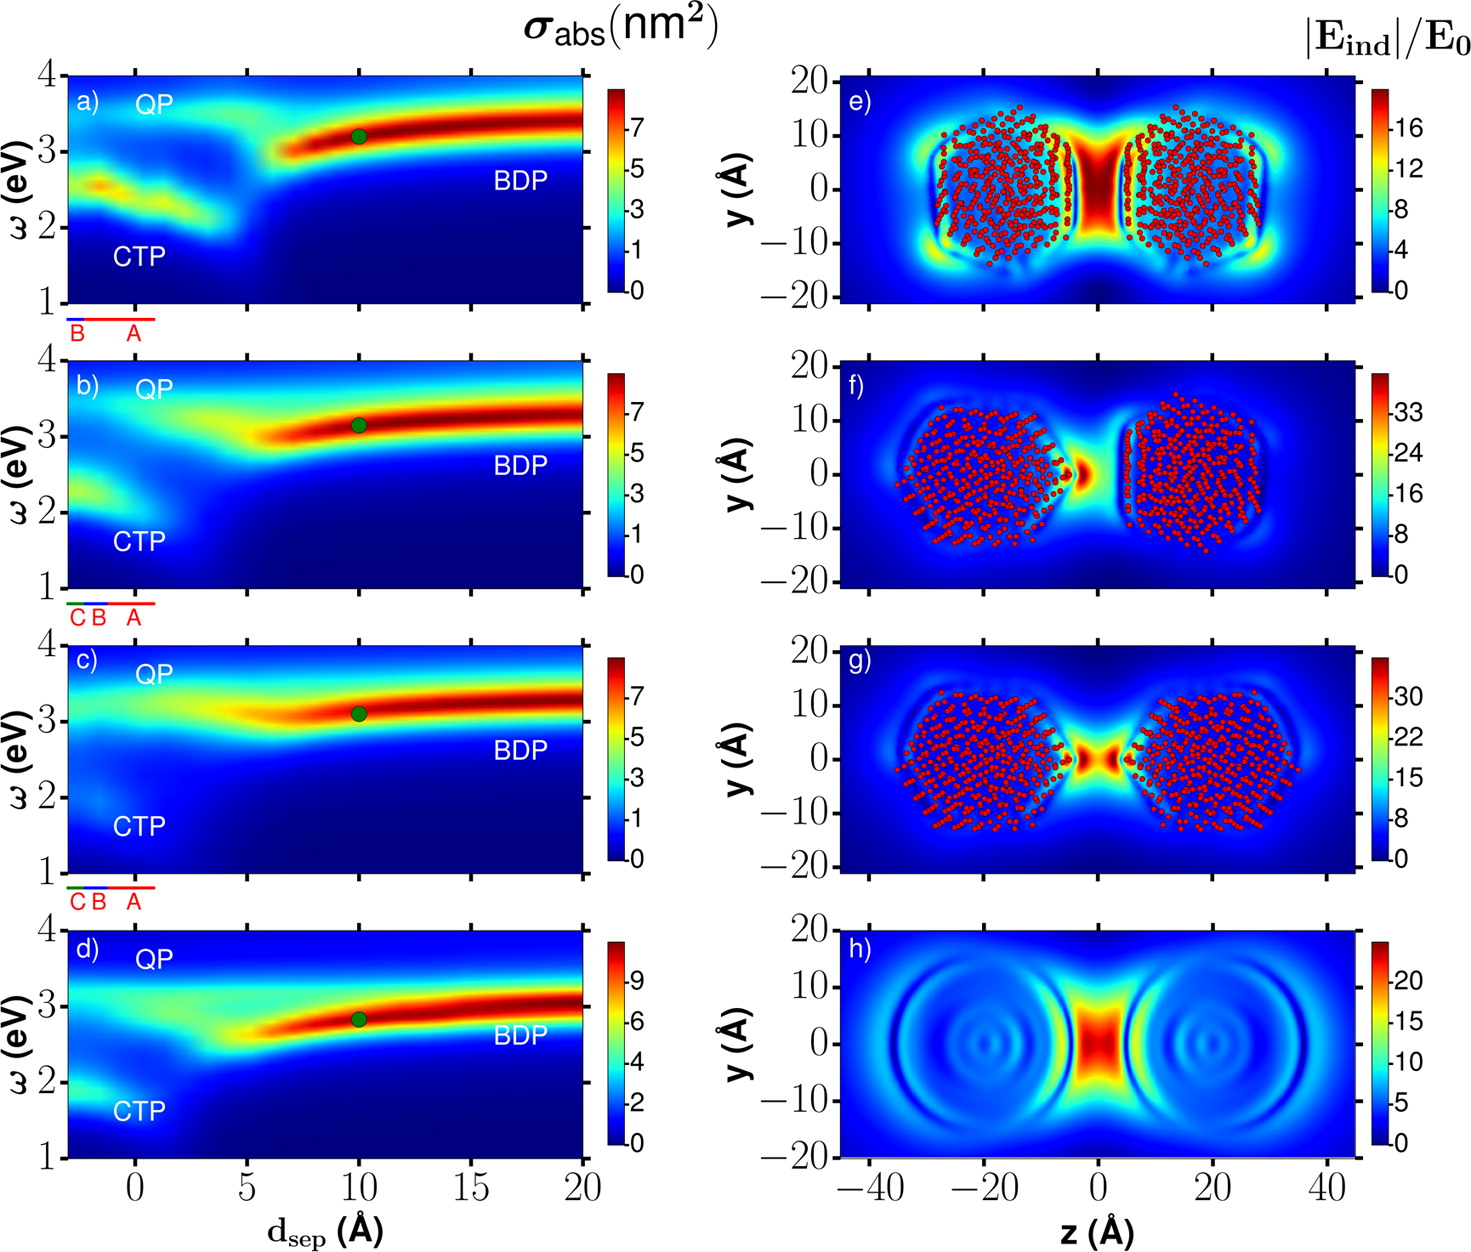
\includegraphics[width=0.6\textwidth]{figures/literature/nl-2015-007593_0001}
\caption[TDDFT calculations of \SI{16}{\angstrom} faceted NaNP dimers arranged with different facet alignments \cite{barbry2015}]{\textbf{TDDFT calculations of \SI{16}{\angstrom} faceted NaNP dimers arranged with different facet alignments \cite{barbry2015}.} Aligned facets leads to the smallest field enhancement and the earliest onset of charge transfer effects at \SI{5}{\angstrom}. Vertex alignment results in an atomic-scale lightning rod effect and increased field localisation. CTP excitation is more difficult in this configuration, occurring at \SI{0}{\angstrom}, due to the small contact but screening is made easier for the same reason, occurring at \SI{7}{\angstrom}. The figure is taken from \cite{barbry2015}.}
\label{fig:atomic_morphology}
\end{figure}

Finally, theory has began to predict the variability of quantum regime plasmonics with gap morphology, showing that atomic rearrangements can dramatically alter the plasmonic response \cite{barbry2015}. This is theoretically demonstrated in \SI{16}{\angstrom} faceted NaNPs dimers in various configurations, shown in \autoref{fig:atomic_morphology}. With flat surfaces aligned the conductance is maximised, with a CTP and a fast blueshift seen as early as \SI{5}{\angstrom}. In contrast, with facet vertices aligned, a CTP only begins to emerge after contact between atoms. Screening in this arrangement is observed earlier at around \SI{6}{\angstrom}, likely due to tunnelling only having to neutralise a small surface area. The facets demonstrate an atomic lightning rod effect that increases the field in the gap whilst minimising the conductance. All other configurations average to the expected result predicted using a spherical particle model. This demonstrates that experiments can in some sense become limited by surface roughness or even atomistic surface defects.

%In theory, this prevents small gaps from being useful as SERS structures but instead provides a method for optically studying electron transport on sub-nm length scales, motivating the need to fully understand these effects.

\subsubsection{Limits of Critical Behaviour in Conductive Plasmonic Nanogaps}

\begin{figure}[bt]
\centering
\vspace{-10pt}
\begin{tikzpicture}
\node [below left] at (0,0) {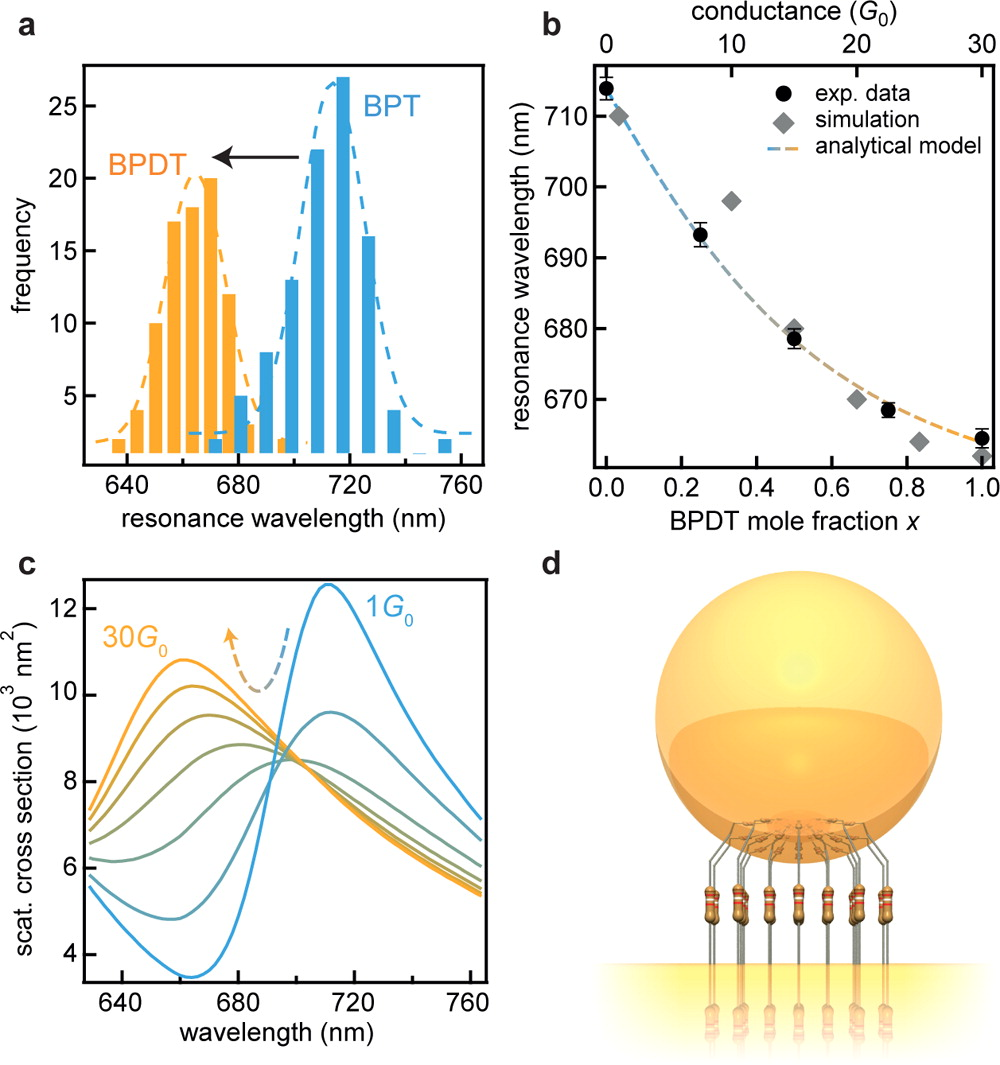
\includegraphics[width=6cm, clip=true, trim=0 125 123 15]{figures/literature/nl-2014-041786_0003}};
\node [below right] at (0,0) {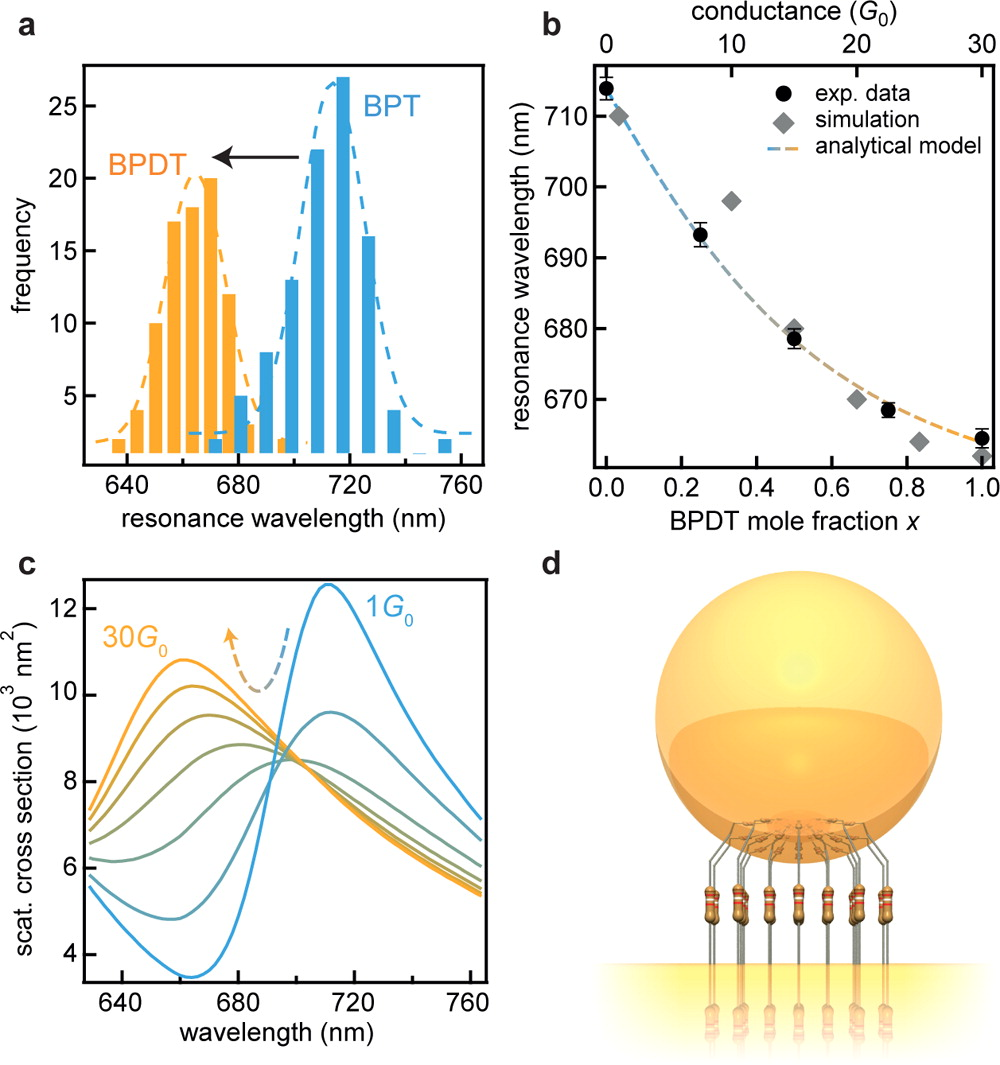
\includegraphics[width=6cm, clip=true, trim=0 4 123 138.5]{figures/literature/nl-2014-041786_0003}};
\node [below left] at (-5.6,0.1) {\textbf{a}};
\node [below left] at (0.7,0.1) {\textbf{b}};
\end{tikzpicture}
\caption[Experimental and theoretical scattering spectra of \SI{80}{nm} AuNP dimers connected via variable conductance molecular linkers \cite{benz2014}]{\textbf{Experimental and theoretical scattering spectra of \SI{80}{nm} AuNP on a planar Au mirror separated via variable conductance molecular spacer layer \cite{benz2014}.} Variable conductance molecular SAMs are formed from fractional mixing of BPT (insulating) and BPDT (conductance). The blueshift and attenuation of the coupled plasmon begins at 2\G0 with the screened mode emerging once $G>5\G0$.}
\label{fig:benz_molecular_npom}
\vspace{-5pt}
\end{figure}

Both the screening-induced blueshift and CTP excitation require a conductance threshold to be surpassed in order for these effects to occur. Thresholds have been defined for a dimer containing a classical conductive linker, where the gap between particles of radius $R$ has a width $d$, conductivity $\sigma$, and linker radius $a$ \cite{perez2010, perez2011}. The blueshift of screened gap plasmons occurs at low conductances with a critical conductance for the dipolar bonding plasmon given by,
\begin{equation}
	G_{\mathrm{SBDP}} = 2\epsfs\omega_{\mathrm{BDP}}\frac{a^2}{d}, \quad \left( \sigma_{\mathrm{SBDP}} = \frac{2\epsfs\omega_{\mathrm{BDP}}}{\pi} \right).
\end{equation}
Reducing the conductance to a conductivity by removing a factor of $\pi a^2/d$ shows that screening is intrinsically independent of geometry and depends only on a critical conductivity. Experiments maintaining a fixed geometry whilst increasing the gap conductivity using fractional mixing of similar conductive and insulating \glspl{sam} have succeeded in showing a blueshift of coupled plasmons with an estimated 2\G0 threshold \cite{benz2014}, as shown in \figurename~\ref{fig:benz_molecular_npom}. A similar 2\G0 threshold is also found in theoretically considered \SI{1}{nm} dimer linkers \cite{perez2010}.

% CTP effect
A second, much larger, threshold exists for CTP formation, occurring at,
\begin{equation}
	G_{\mathrm{CTP}} = \epsfs\omega_{\mathrm{CTP}}\frac{R^2}{d}, \quad \left( \sigma_{\mathrm{CTP}} = \frac{\epsfs\omega_{\mathrm{CTP}}}{\pi} \left(\frac{R}{a}\right)^2 \right).
\end{equation}
Unlike screening, CTP formation depends not only on the conductivity but also the junction geometry. The geometrical factor $(R/a)$ represents the ratio between the total charge in the particle and the amount which can pass through a gap with fixed conductivity. Hence, a small, nanometre-scale but highly conductive junction between particles can accommodate sufficient current to maintain a CTP. This has been experimentally demonstrated in AuNP dimers separated by hollow spacer molecules and linked by a Au thread during exposure to high power laser pulses \cite{herrmann2014, tserkezis2014}.

Interestingly, qualitative agreement between QCM calculations and full quantum mechanical calculations suggest that the quantum nature of the system is of little importance. Even though the QCM uses a classical, resistive gap with conductance values characteristic of quantum transport, quantum effects on gap plasmons are accurately replicated. This implies that, despite the quantum nature of such small gaps, the effects on plasmon coupling only depend on the amount of charge transfer and not the mechanism by which it occurs. This links together work done using particle positioning \cite{savage2012, scholl2013} with studies of interacting plasmonic system coupled with molecular linkers \cite{tan2014, cha2014, benz2014}. Quantum tunnelling and quantised conductance still remain interesting cases, however, since both forms of conduction are unavoidable once gap sizes decrease below \SI{0.5}{nm}. This is why the point at which the electric field is expelled from the gap is described as the quantum limit to plasmon confinement \cite{savage2012}. For this reason, it is important to fully understand the relations between plasmonic hot spots and sites of (quantum) charge transfer.

\end{document}